\documentclass[letterpaper]{article}
\usepackage[utf8]{inputenc}
%\usepackage[latin1]{inputenc}
\usepackage[spanish]{babel}
\usepackage{geometry}
\usepackage{anysize}
\usepackage{graphicx} 
\usepackage{amsmath}
\usepackage{float}
\usepackage{xy}
\usepackage{color}
%\numberwithin{equation}{list}
\marginsize{1cm}{2cm}{0cm}{2cm}  
\title{Problema a cuenta del Parcial 1 \\ \begin{large}Curso de Física Computacional\end{large}}
\author{M. en C. Gustavo Contreras Mayén}
\date{ }
\begin{document}
\maketitle
\fontsize{14}{14}\selectfont
\spanishdecimal{.}
Considera la siguiente imagen:
\begin{figure}[H]
	\centering
	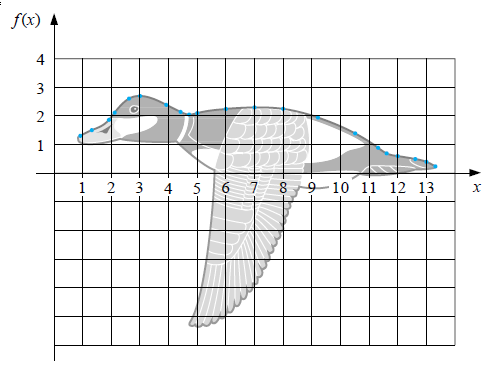
\includegraphics[scale=1.3]{Imagenes/ContornoPato.png} 
\end{figure}
Encuentra una función que represente el contorno del pato en el primer cuadrante, para ello debes:
\begin{enumerate}
\item Definir un conjunto de puntos (entre 20 - 25 puntos)
\item Revisa si la función de interpolación representa debidamente el contorno del pato:
\begin{enumerate}
\item Con la técnica de interpolación de Lagrange.
\item Con la técnica de interpolación con splines.
\end{enumerate}
\item Entrega tu código en python y gráficas correspondientes.
\end{enumerate}
Discute tus resultados.
\end{document}